\section{简介}

如图~\ref{fig:overview},以C++为基本,对基础部分进行学习。
了解C++基本语法,学习类与数据对象,容器和算法,\textbf{面向对象和泛型编程(重点)},编译与底层,C++新特性。

\begin{figure}[]
	\centering
	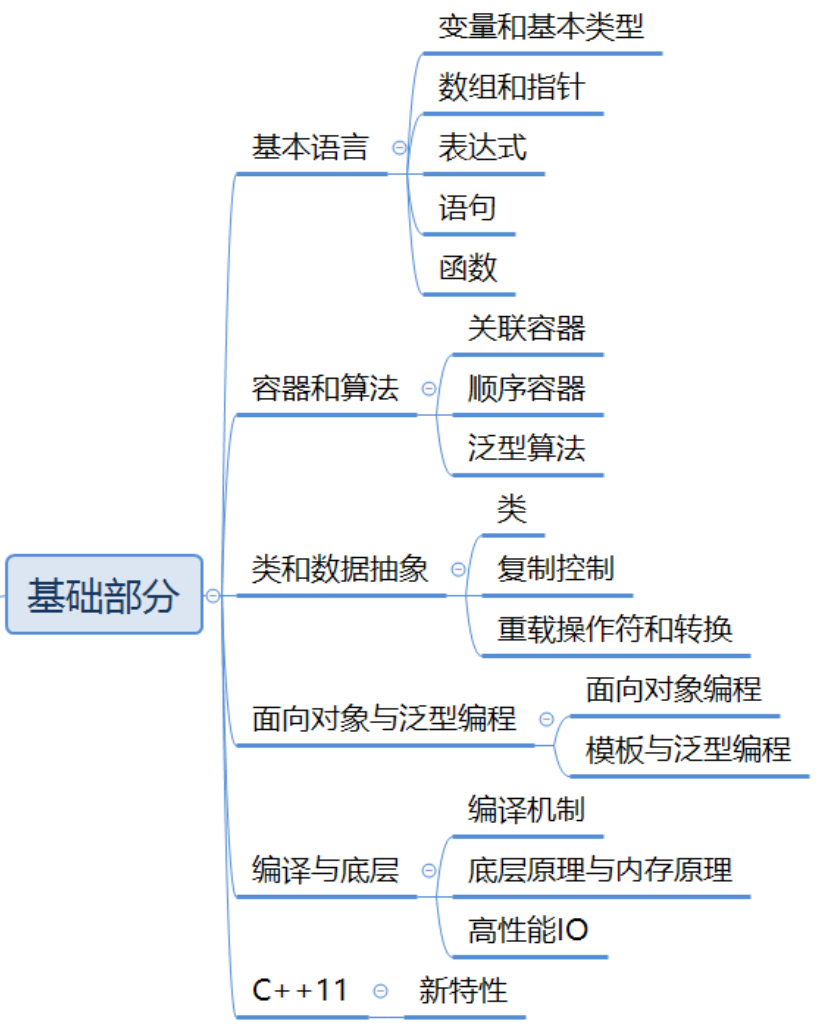
\includegraphics[width=0.5\columnwidth]{pic/overview.png}
	\caption{基础部分学习总览}
	\label{fig:overview}
	% \vspace{-5pt}
\end{figure}

\section{C++ Review}
C++语言同时支持五种编程风格:C风格(面向过程)、基于对象、面向对象、泛型和函数式。
在C++11之前抽象存在若干的缺陷,最严重的是缺少自动内存管理和对象级别的消息发送机制。
现代C++语言可以看作是三部分组成的:1.低级语言,大部分继承自C;2.现代高级语言特性,允许我们定义自己的类型以及组织大规模程序和系统;3.标准库,利用高级特性来提供有用的数据结构和算法。
\begin{tcolorbox}[boxsep=-0.05in]
	\underline{C++和C有什么区别:} C++有与C一样的低级语言特性,面向过程,这部分主要继承于C;同时C++,尤其是C++11拥有众多的高级语言特性,使得程序更加易于开发,提供非常多的标准库,使得实现特定的数据结构和算法更加简单。同时,C++相比于C,它支持更多的编程模式,比如面向对象,基于对象,函数式编程以及泛型编程。
	\textbf{参考答案:}设计思想上,C++是面向对象的语言,而C是面向过程的结构化编程语言;语法上,C++具有封装、继承和多态三种特性,C++相比C,增加多许多类型安全的功能,比如强制类型转换、C++支持范式编程,比如模板类、函数模板等。
\end{tcolorbox}

\subsection{C++基础}
\begin{itemize}
	\item \textbf{输入输出流:} iostream,$cin >>$, $cout <<$。
	\item \textbf{控制流:} while(condition) {statement} ; for(int i=1;i<=10;++i){statement} ; if(condition){statement};
	\item \textbf{基本内置类型:} 算术类型(整形(包括字符和布尔)|浮点型):bool, char, wchar\_r, char16\_t, char32\_t, short, int, long, long long, float, double, long double。 bit(1)-byte(8)-word(32/64) byte是寻址的最小内存单元。无符号数永远不会小于零,切勿混用。'a'单引号是char型字面值,"hello"叫字符串字面值,字符串型字面值结尾会补一个空字符。
	\item \textbf{初始化和赋值}要加以区分,但事实上无关紧要。赋值是将对象的当前值擦除,而以新值代替。建议初始化所有的内置类型的变量。
	\begin{lstlisting}[caption={}]
		int units = 0;
		int units = {0};
		在C++11中用花括号初始化变量得到了全面的应用,该形式称为列表初始化。该方式在赋值中如何会
		丢失值(非强制类型转换),编译器会报错。
		int units{0}; 
		int units(0);
	\end{lstlisting}
	\item \textbf{extern} 为了支持分离式编译,C++将声明和定义区分开来。声明只是让名字为程序所知,而定义负责创建与名字关联的实体。在实际执行上,定义申请存储空间,也可能会赋初值,而声明不会。 extern int i; int j; 但是extern int i = 1;是声明,因为包含了显示初始化。变量能且只能被定义一次,但是可以被多次声明。主要用来解决多个文件中使用同一个变量的情况。
	\item \textbf{复合类型}指基于其他类型定义的类型,如引用和指针。一般情况下说引用就是指左值引用,而在C++11中新增了右值引用。类型修饰符放在名字之前,而不是数据类型一起不容易产生误导。
	\item \textbf{引用} int ival = 1024; int $\&$ref = ival;引用必须被初始化。引用即别名,且只能绑定一次,相当于又起了一个名字。注意,不能定义引用的引用,因为应用本身不是一个对象。
	\item \textbf{指针} int ival = 42; int * p = \&ival; \&取地址符。 $cout << *p$; *是访问指针所指的对象,叫解引用符。
	\item \textbf{空指针} 不指向任何对象,因此编程中在使用一个指针之前要先判断其是否为空。nullptr(C++11) NULL 0; NULL叫做预处理变量,在cstdlib中定义,它的值就是0。
	\item \textbf{void*指针} 可用于存放任意对象的地址。但是void*不记录对象类型,因此不能用其操作/访问对象,只能比较地址或者作为返回值(传递)。
	\item \textbf{指向指针的指针} 指针与引用不同,是内存中的对象。因此可以有指向指针的指针。int **ppi = \&pi;同时可以有指向指针的引用; int* \&r = p; int* 说明引用的类型,而\&说明它的本质是引用,此时r就是p的一个别名,直接和p一样用就可。遵循从右向左解释。
	\item \textbf{const限定符} const int bufSize = 512; 缓冲区大小,且不能改变,只能访问内容,不能修改。在编译过程中,编译器会将所有的bufSize都直接换成512。为了避免对同一变量的重复定义,默认情况下,const对象被设定为仅在文件内有效。当多个文件中出现同名的const变量时,其实是不同的独立定义了变量。当有必要在文件之间共享,而不是编译器为每个文件生成独立的变量时候,只需要在一个文件中定义const,而在多个文件中声明。全部加上extern关键字,只在一个地方初始化即可。
	\item \textbf{const的引用} 可以引用,但是不能通过引用修改对象,因此它还是一个常量。const int i = 1; const int \& ri = i;
	\item \textbf{常量引用的非常量对象} int i = 42; const int \&r1 = i; const int \&r2 = 42; const int \&r3 = r1*2; 总之引用的限制条件必须大于右边进行初始化的量。
	\item \textbf{指向常量的指针} 令指针指向常量或非常量。 const double * pi = 3.14。类似的,左边的限制条件必须大于右边。
	\item \textbf{常量指针} int *const p; 因为指针本身是对象,因此允许将指针本身定义为常量,不变的是指针的值,而非指向的那个值。\textbf{顶层const} top-level const表明指针本身是个常量,\textbf{底层const} low-level表明指针所指的对象是一个常量。
	\item \textbf{常量表达式}指在编译阶段就能知道计算结果的表达式。c++11中运行将变量声明为constexpr类型提示编译器。constexpr int mf = 20;对于类型比较简单,值也显而易见的称为字面值类型。
	\item \textbf{typedef} typedef double *p; p 就是double*; 在C++11中定义了一个新方法:using SI = Sales\_item; 当对指针时候,注意区分指向常量的指针和常量指针。
	\item \textbf{auto} auto item = v1 + v2; auto定义的变量必须有初始值。在一行中定义多个变量用auto时需要注意,因为auto只有一个,当初始值赋值可能判断为不同的类型,会报错。
	\item \textbf{decltype} decltype(f()) sum = x; 判断f()返回的类型,作为sum的类型。当涉及到引用的时候还挺麻烦。如decltype((i))返回的就是一个引用类型。
	\item \textbf{struct自定义数据类型} struct Sales{std::string bookNo; unsigned units = 0; double revenue = 0.0;};
	\item \textbf{头文件} 像是一个声明,类通常被定义在头文件中,类所在的头文件的名字应与类的名字一样。头文件通常包含那些只能被定义一次的实体,如类、const、和constexpr变量。
	\item \textbf{头文件保护符} 为了不多次包含相同的头文件,通常需要$\#$ifndef SALES\_DATA\_H $\#$define SALES\_DATA\_H $\#$include <string> $\#$endif。预处理变量无视作用域规则。	
\end{itemize}

\subsection{字符串、向量和数组}
上一小节介绍的是内置类型,这一节是抽象数据类型库。其中string和vector是两种最重要的标准库类型,string支持可变长字符串,vector支持可变长的集合。

\textbf{using} using std::cin; using namespace::std; 头文件不应该包含using声明,防止被放在不同文件中出错。

\subsubsection{String}
string对象上的操作:
\begin{itemize}
	\item \textbf{$os << s$} 将s写到输出流os当中,返回os. 注意输入输出都以空格结束,即一有空格就算作下一个字符串了。
	\item \textbf{$is >> s$} 从is中读取字符串付给是,字符串以空白分割。
	\item \textbf{getline(is,s)} 从is读取一行付给s,返回is。
	\item \textbf{s.empty()}是为空返回true,否则返回false。注意这里所有的返回值都是string::size\_type,不算int啥的,因此最好用 decltype(s.size()) n = s.size()
	\item \textbf{s.size()}返回s中字符的个数。
	\item \textbf{s[n]}返回s中第n个字符的\underline{引用},位置n从0记起。有点儿像切片
	\item \textbf{s1+s2}字符串相连。
	\item \textbf{s1=s2}以s2替换s1。
	\item \textbf{s1==s2}判断相等,相等性对大小写敏感。对于比较,则利用字符在字典中的顺序,对大小写敏感
	\item \textbf{cctype}处理string对象中的字符,可以用到cctype头文件,判断大小写,标点符号,十六进制,是不是空格,可不可以打印,字母还是数字。注意,尽可能的使用C++版本的头文件,前面多个c,且去掉了.h后缀。
	\item \textbf{对于输出字符串中的每一个字符} $for(auto c : str) cout << c <<endl;$注意如果向改变str中的值,必须把c定义成引用。当用引用时,这里其实是将c一次绑定到str上的每个字符,操作c就是操作了str,否则就无法改变str。
	\item \textbf{下标运算符} str[1] 返回的是对位置1的引用。访问字符串之前,最好先.empty()一下。
\end{itemize}

\subsubsection{Vector}
vector是一个类模板,对于类模板需要将指定模板实例化成什么样的类,需要提供哪些信息由模板决定。提供信息的方式是尖括号,如$ vector<int> ivec; vector<vector<int>> ivvec; $
\begin{itemize}
	\item \textbf{初始化}vector<int> ivec(10, -1);  还有列表初始化等。
	\item \textbf{向vector对象中添加元素} v.push\_back(i); 这里vector额外提供了方法,允许我们进一步提升动态添加元素的性能。
	\item \textbf{循环体内部有向vector添加元素的语句,则不能使用for循环} 这是因为vector是动态变化的,内存不够用的时候会自动开辟新内存,导致其下标指向的元素也会随着vector添加元素的数量动态变化。
	\item \textbf{v.empty()}
	\item \textbf{v.size()}
	\item \textbf{v[n]}
	\item \textbf{v1 = v2}
	\item \textbf{v1 = {a,b,c...}}
	\item \textbf{v1 == v2}
	\item $vector<int>::size\_type$
	\item \textbf{不能用下标形式添加元素} 因为vec里其实是不包含任何元素的。只能push\_back()
\end{itemize}

\subsubsection{Iterator迭代器}
除去下标方式,也可以用迭代器的方式。所有标准库容器都可以使用迭代器。对于有迭代器的类型,同时就拥有返回迭代器的成员。 auto b = v.begin(); auto e = v.end(); end()一般用来判断迭代器是否到头。同时对于不需要写的操作,也定义有v.cbegin(),返回const\_iterator类型的对象。

迭代器的运算符:
\begin{itemize}
	\item \textbf{*iter} 返回所指元素的引用。(不是引用就没办法对其进行修改)
	\item \textbf{iter->mem} 获取该元素的mem成员,等价于(*iter).mem
	\item \textbf{++iter}
	\item \textbf{--iter}
	\item \textbf{iter1==iter2}
	\item \textbf{迭代器类型}一般是iterator或者const\_iterator
	\item \textbf{迭代器解引用} 可获得迭代器所指的对象,如果该对象的类型恰好是类,就有可能希望进一步访问它的成员。(*it).empty() it是某个容器的迭代器,用(*)解引用然后进行操作,注意()是必须的,否则‘.’运算符将由it来执行。或者it->empty(),箭头运算符直接获取容器对应的方法。
	\item \textbf{迭代器运算} iter+n 移动n步;iter += n将迭代器移动n的结果赋给iter;iter2-iter1两个迭代器之间的距离。
\end{itemize}

\begin{tcolorbox}[boxsep=-0.05in]
	迭代器中往往采用v.begin() != v.end()来判断是否为空,而非大于号小于号,这是因为迭代器中往往只定义了!=操作,更符合C++程序员的习惯。
\end{tcolorbox}

\subsubsection{数组}
与vector类似的数据结构,在性能上优于vector,但是在灵活性上差,如果事先不能确定元素的确切个数,用vector。int a[10]; int * pa[10];string str[10]; 定义的时候必须有具体维度。同时也不存在引用的数组。也不能用auto。char a4[] = "C++"; 注意双引号括起来的数组最后隐含一个空字符。
\begin{itemize}
	\item \textbf{存放指针的数组} int *ptrs[10];
	\item \textbf{数组的指针} int (*Parray)[10] =\&arr; 指向一个含有10个整数的数组;这里理解起来就是有一些特异性,先声明是个指针,再说明是一个指向包含10个元素的数组的指针。
	\item \textbf{数组的引用} int (\&Rarray)[10] = arr; 引用一个含有10个整数的数组;
	\item int *(\&arry)[10]=ptrs;arry是一个引用,引用的是一个包含10个元素的指针数组。理解数组,从数组名字开始由内到外阅读。
	\item \textbf{指针与数组} string nums[]={"one","two","three"}; string *p = nums; string *p=\&nums[0]; 指针也是迭代器。
	\item \textbf{数组的begin end} int *beg = begin(nums); 由于数组不是类类型,C++11提供了两个新函数完成这个工作。
\end{itemize}

\subsubsection{多维数组}
多维数组只是数组的数组。引用和多维数组与指针和多维数组差不多。指针 ++p,是在对应维度进行指针的递增,这也印证了多维数组只是数组的数组。
\begin{itemize}
	\item int arr[10][100][1000] = {};
	\item {范围for循环}是在C++11中新加的。
	\begin{lstlisting}[caption={}]
		size_t cnt = 0;
		for (auto &row : ia)
			for (auto &col : row){
				col = cnt;
				++cnt;
			}
	\end{lstlisting}
\end{itemize}

\subsubsection{C风格字符串}
最好别用,要用就用标准库string。cstring 是 string.h 的C++版本。

\subsubsection{与旧代码的接口}
\begin{itemize}
	\item 为了\textbf{兼容C风格字符串},C++提供了 string.c\_str成员函数,来把值付给 char *str。也就是const char *str=s.c\_str();
	\item \textbf{使用数组初始化vector对象} 不允许数组为另一个内置对象赋初值,也不允许使用vector对象初始化数组,相反的,允许使用数组来初始化vector对象。int int\_arr[] = {0,1,2,3,4};$vector<int> vi(begin(int\_arr)+1,end(int\_arr));$ 反正只要传入两个指针就可。
\end{itemize}

\subsection{表达式}
\subsubsection{基础}
\begin{itemize}
	\item 一元运算符,二元运算符
	\item \textbf{重载运算符},当运算符用于类类型的运算对象时,可以重载。
	\item \textbf{左值和右值} 当一个对象被用作右值的时候,用的是对象的值(内容);当对象被用作左值的时候,用的是对象的身份(在内存中的位置)。一个原则是当需要用到右值的地方可以用左值替代,但不能反过来,左值永远可以获取到对应的右值。
\end{itemize}

\subsubsection{算术运算符}
+ - * / \%  

\subsubsection{逻辑和关系运算符}
$! > < <= >= != == \&\& || $

\subsubsection{赋值运算符}
= 左侧必须是一个可修改的左值。赋值运算符优先级较低。

\subsubsection{递增和递减运算符}
++ --

前置版本:先做加减运算,然后将改变后的值作为求值结果。
后置版本:先有一个副本作为求值结果,在加减运算。除非必须,否则不用。

\subsubsection{成员访问运算符}
->
\subsubsection{条件运算符}
cond ? expr1 : expr2;

\subsubsection{位运算符}
bitset的标准库。内置运算符。移位运算符是其重载。
\begin{itemize}
	\item ~位求反
	\item $<<$ 左移
	\item $>>$ 右移
	\item \& 位与
	\item 位异或
	\item $|$ 位或
\end{itemize}

\subsubsection{sizeof运算符}
返回所占的字节数。

\subsubsection{隐式转换/显示转换}
$cast-name<type>(expression);$ 一般别用。

$ slope = static\_cast<double>(j) / i;$只要没有底层const就可以用。一个用法是用其找回存放在void*中的指针值。

const\_cast只用于改变运算对象的底层const。再次确认 const char * 和 char *是两个类型。const和char是一体的。

reinterpret\_cast通常位运算对象的位模式提供较低层次上的重新解释。一般不用。

\subsection{语句}

\begin{itemize}
	\item \textbf{if} if (cond) statement if else
	\item \textbf{switch} switch(ch) {case 1: break; case 2: break; default: break;}
	\item \textbf{while} 
	\item \textbf{for} 传统for和范围for。传统for的定义变量可以定义多个,但必须都是同样的类型。范围for主要用来遍历容器和其他序列的所有元素。
	\item \textbf{do while} do statement while(condition);
	\item break和continue。
	\item goto 别用。
	\item try语句和异常处理。
	
	$\#include <stdexcept>$
	
	throw表达式来抛出异常。throw runtime\_error("it is wrong");
	try+cactch捕捉异常。
	一套异常类(expression class)用于在catch和throw之间传递消息。
	\begin{lstlisting}[caption={}]
	try {
		if()
		throw runtime\_error("it is wrong"); 被第二个catch捕获。
	} catch(exception-declaration){
		handler;
	} catch(runtime_error err){
		error.what() 输出error的内容
	}
	\end{lstlisting}
	\item 具体异常类可见书P176。
	
	
\end{itemize}

\subsection{函数}
\begin{itemize}
	\item 函数定义的地方叫形参,调用叫实参。
	\item 函数调用完成两项工作:一个是用实参初始化形参,二是将控制权转移给被调用的函数。主调函数被终端,被调函数开始执行。
	\item 名字有作用域,对象有生命周期。
	\item \textbf{局部静态对象} static size\_t ctr = 0;在函数结束之后仍然存在。
	\item \textbf{函数声明} 在头文件中进行函数声明,在源文件中定义。
	\item 当初始化一个非引用类型的变量时,初始值会被拷贝给变量,但是对变量的改动不会影响初始值。
	\item 使用引用和指针,避免拷贝。使用引用形参返回额外信息。
	\item \textbf{const形参和实参} 和赋值时遵循一样的规则。为了能把const的值传进函数,对于不会改变的形参,尽可能的定义为const。
	\item \textbf{数组引用形参} 切记是 int (\&arr)[10]; 括起来表达的是一个引用,不括是引用的数组。
	\item \textbf{int main(int argc, char *argv[]);}
	\item \textbf{含有可变形参的函数} 
	
	1. 如果函数的实参数量未知,但是全部实参的类型都相同,使用initializer\_list类型的形参(一种标准库类型)。$void error\_msg(initializer\_list<string> li)$。类似vector。
	
	2. 省略符形参,这个主要是为了方便C++程序访问C代码,使用了varargs的C标准库功能。void foo(para\_list, ...);
	\item 返回类型和return语句。返回引用的时候是个左值,可以放在等号的左边。就是刚刚返回就被改变了,不会有人这样用。
	\item 主函数main可以没有返回值。
	\item 递归函数
	\item \textbf{返回数组指针} int (*func(int i))[10];
	\item 尾置返回类型 auto func(int i) -> int(*)[10];
	\item \textbf{函数重载} 函数名字相同,但是形参不同。
	\item 重载必须声明在同一级作用域上,不然就可能出错。
	\item 也可以有默认实参。多次声明中,一个形参只能有一次默认实参。
	\item \textbf{内联函数inline}。调用函数一般比求等价表达式值要慢一些,因为调用包含拷贝之类的过程。而内联函数在调用点“内联的”展开。只需在函数返回类型前面加上关键字inline。一般函数一般用于规模较小,频繁调用的函数。
	\item \textbf{constexpr函数}是指能用于常量表达式的函数,函数的返回类型以及所有的形参的类型都得是字面值。constexpr隐式的被定义为内联函数。
	\item 内联函数和constexpr函数通常定义在头文件中。
	\item \textbf{assert 和 NDEBUG预处理宏} 可以用于屏蔽调试代码。
	
	assert(expr)首先对expr求值,如果为假,则assert输出信息病终止程序。话说这个东西不是叫断言么。assert定义在cassert头文件中。
	
	NDEBUG预处理变量,如果定义了$\#define NDEBUG$则不执行assert,或者g++ -D NDEBUG也可以。
	或者$\#ifdef NDEBUG xxxx \#endif$
	
	此外,\_ \_FILE\_ \_ \_ \_LINE\_ \_ \_ \_TIME\_ \_ \_ \_DATE\_ \_分别定义了文件名,当前行号,编译时间,编译日期。
\end{itemize}

\subsubsection{函数匹配}
确定调用选择哪个重载函数。

\subsubsection{函数指针}
函数的类型由它的返回类型和形参类型共同决定,与函数名无关。

对于 bool lengthCompare(const string \&, const string \&);他的类型是

bool(const string \&, const string \&);

对应的指针是 bool (*pf)(const string \&, const string \&);其中括号必不可少,不然就是一个返回值是bool指针的函数。

pf=lengthCompare;

bool b1 = pf("Hello","goodbye");

bool b2 = *pf("Hello","goodbye");两者等价,不必解引用也可以。

重载函数必须清晰界定是哪个函数。

void useBigger(const string \&s1, const string \&s2, bool (pf)(const string\&, const string \&));

void useBigger(const string \&s1, const string \&s2, bool (*pf)(const string\&, const string \&));

\subsection{类}

数据抽象和封装,数据抽象依赖于接口和实现,封装实现了类的接口和实现的分离。

\begin{itemize}
	\item 利用public和private访问说明符,为类添加封装性。
	\item 使用关键字class定义类。struct和class都可以,唯一区别是默认访问权限不一样。在第一个访问说明符之前,struct关键字下是public的,而class的是private的。class是以private为主。
	\item \textbf{友元}。类允许其他类或者函数访问它的非公有成员的方法。在类中用friend关键字声明友元函数。
	\item 最好还是在类的外部提供一个独立的声明。
	\item 成员函数也可以被重载。
	\item \textbf{mutable}一个可变数据成员永远不会是const,即使他是const对象的成员。对于 void func() const{}函数是一个只读函数,但是对于有mutable声明的变量,也可以修改。
	\item C++11, 类内初始值。
	\item 返回*this的成员函数,return*this,就可以 myScreen.move(4,0).set("#").
	\item 类类型,即使成员函数完全一样,不同的类就是不同的类型。
	\item 类声明。
	\item 可以把其他类定义成友元,也可以把其他类的成员函数定义为友元. friend class Windows\_mgr; friend void Window\_mgr::clear(ScreenIndex)
	\item \textbf{委托构造函数}.算是语法糖吧,没啥意思.
	\item 在实际中,如果定义了其他构造函数,最好也提供一个默认构造函数.
	\item 可以在类成员函数前添加\textbf{explicit}禁止隐式的数据类型转换.
	\item 当一个类,1. 全部的成员都是public的,2. 没有定义任何构造函数, 3. 没有类内初始值, 4.没有基类,没有virtual函数,就叫\textbf{聚合类}.可以直接初始化.
	\item \textbf{static}静态成员,静态成员存在于任何对象之外,为类的所有对象所共享. static只出现在类的内部.
\end{itemize}

\subsection{IO库}
C++不直接处理输入输出,而是定义了标准库来处理IO,这些类型支持从数据读取,向设备写入.设备可以是文件,控制台窗口.
区别于第一章进行记录.iostream定义了用于读写流的,fstream定义了读写文件,sstream读写内存string对象的类型.

ifstream和istringstream都是继承自istream的. 因此在调用上是一样的.

IO操作容易发生错误,有时候也需要知道为什么发生错误,然后选择正确的处理方式,因此iostream提供了流状态的查询.发生错误了就用setstate把对应位置置位,然后cin.eof()等函数查看到底是怎么错的,继续做.
\begin{lstlisting}[caption={}]
	auto old\_state = cin.rdstate();
	cin.clear(); 复位
	process_input(cin);
	cin.setstate(old\_state); 表示发生对应错误
	cin.clear(cin.rdstate \& ~cin.failbit \& ~cin.badbit); ~是位求反.
\end{lstlisting}

endl, flush, ends, unitbuf, nounitbuf,

打开文件可能出错,因此if(file),检查一下是对的,其实就是检查前文的rdstate,有一个错,就是错.应该是与操作.不同的错误发生相应的置位.

in读模式,out写模式,app每次写定位到文件末尾,ate打开文件后立即到文件末尾,trunc截断文件,binary以二进制方式打开文件io. 可以指定多个模式.

\textbf{String流}定义了三个类型来支持内存IO,把string当作一个IO流.

\subsection{顺序容器}

vector

